\section*{Metodología}
Durante el desarrollo del proyecto se estructuró un proceso reproducible para estimación 
de precios de vivienda que incluyó: 

% TODO: Usar una lista ordenada
(i) adquisición y validación de datos, 
(ii) limpieza con reglas explícitas para mitigar sesgos por valores extremos y errores de captura,
(iii) entrenamiento de modelo de linea base, 
(iv) enriquecimiento geoespacial con capas oficiales y POIs, 
(v) entrenamiento y evaluación de modelos con validación cruzada,
(vi) cálculo de valores estadísticos agrupados para enriquecer resultados, 
(vii) persistencia de artefactos y exposición mediante API. 


% TODO: incorporar información a cerca de la selección de la metrica de error RMSE, por su interpretabilidad y su unidad (pesos colombianos)


\begin{figure}[h]
    \centering
    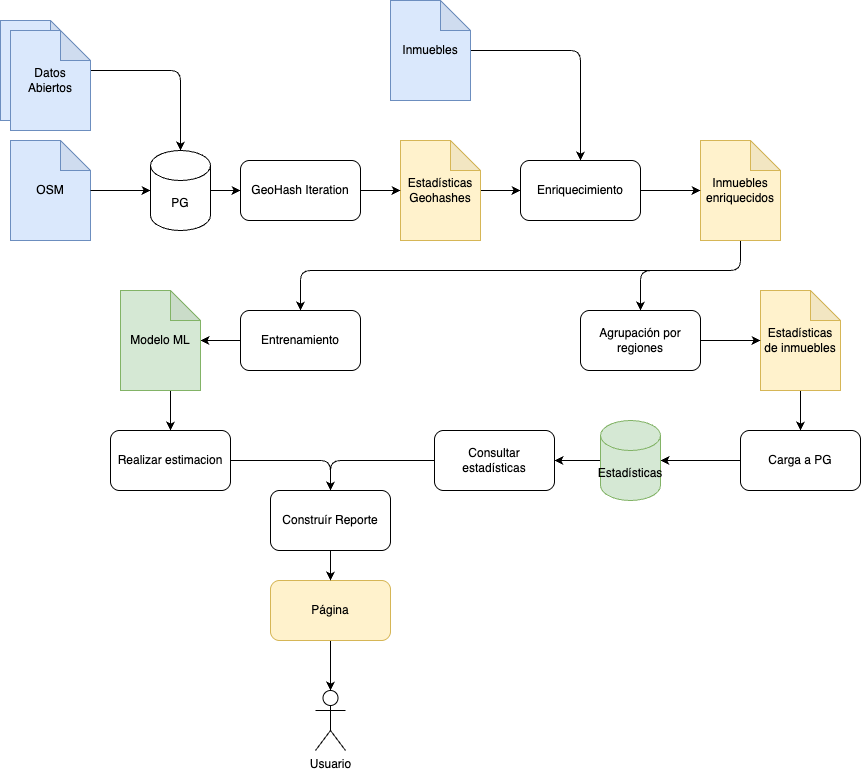
\includegraphics[width=0.85\linewidth]{Images/metodologia.png}
    \caption{Proceso general de la metodología}
    \label{fig:metodologia}
\end{figure}

\subsection*{Fuentes de datos}
Se integraron fuentes públicas y abiertas. 
Los datos de inmuebles proveen variables estructurales, mientras que las capas distritales y POIs agregan contexto espacial y de accesibilidad.
\begin{itemize}
    \item \textbf{Datos de inmuebles (base)}: JSON único de agosto de 2024 publicado en GitHub (\texttt{builker-col/bogota-apartments}). Se transformó a CSV para su análisis.
    \item \textbf{Datos abiertos del distrito (PostGIS)}: Se obtuvieron capas desde la web de datos abiertos del Distrito \cite{datosabiertos_bogota} 
    (consultada en julio de 2025), estos archivos fueron descargados en formato .shp y 
    luego fueron cargados como capas en postgis mediante un script de importación, las capas
    descargados fueron las siguientes: \texttt{barrios\_bogota}, \texttt{upz\_bogota}, 
    \texttt{localidades\_bogota}, 
    \texttt{estratos\_manzana}, \texttt{avaluo\_catastral\_manzana}, 
    y POIs OSM (\texttt{gis\_osm\_pois\_free\_1}\allowbreak, \texttt{gis\_osm\_pois\_a\_free\_1}).
    \item \textbf{Puntos de interés (POIs)}:
    Los puntos de interés cercanos se obtuvieron a partir de datos de OpenStreet map, 
    descargados desde la página web de Geofabrik \cite{geofabrik}.
\end{itemize}



\subsection*{Limpieza y preprocesamiento}
Se normalizó la calidad del dataset para reducir la influencia de colas largas y errores de captura. Se imputaron valores faltantes preservando coherencia estructural entre variables comparables. El proceso se ejecutó en Python (\textit{Pandas}, \textit{NumPy}, \textit{scikit-learn}).
\begin{itemize}
    \item \textbf{Outliers}: filtro por percentil 99. \emph{Área} \(\leq 464\,m^2\), \emph{precio\_venta} \(\leq 5{,}4\times 10^9\) COP.
    \item \textbf{Precio mínimo}: \(\geq 50{,}000{,}000\) COP.
    \item \textbf{Área igual a 0}: imputación por mediana de comparables (mismo \emph{estrato}, \emph{habitaciones}, \emph{banos}, \emph{sector}); si no hay, mediana por \emph{estrato}.
    \item \textbf{Parqueaderos negativos}: reemplazo por moda dentro del mismo \emph{estrato} (sino, moda global).
    \item \textbf{Coordenadas}: imputación por mediana del \emph{sector} o global cuando estén fuera de Bogotá; bounding box final: lat \([4.4, 4.9]\), lon \([-74.3, -73.9]\). Registros fuera se eliminan tras imputación.
    \item \textbf{Estrato fuera de rango [1--6]}: imputación por modo del \emph{sector}; si no hay, modo global.
\end{itemize}

\subsection*{Modelos base}
Se evaluaron varios algoritmos con una misma estrategia de preprocesamiento para asegurar comparabilidad. La validación cruzada controló varianza y evitó sobreajuste; la métrica principal fue RMSE en escala real.
Preprocesamiento: \texttt{SimpleImputer} (media/moda), \texttt{StandardScaler}, \texttt{OneHotEncoder}. Resultados (aprox.):
\begin{itemize}
    \item \textbf{Random Forest}: RMSE \(\approx\) 245M (CV); en\ hold-out (20\%): RMSE \(\approx\) 250.6M, MAE \(\approx\) 129.9M, R\textsuperscript{2} \(\approx\) 0.915.
    \item \textbf{XGBoost / LightGBM}: RMSE \(\approx\) 245--246M (CV).
    \item \textbf{Lineales}: \(\approx\) 348M; \textbf{SVR}: \(\approx\) 913M.
\end{itemize}
Se evaluó además con \(\log(\textit{precio\_venta})\) y \(\log(\textit{area})\), mejorando métricas en escala original.


% TODO: Inicio de creación del modelo aumentado

\subsection*{Uso de Geohash}
Para optimizar el cálculo de puntos cercanos, se utilizó el geohash con un nivel de precisión que 
asegurara una granularidad adecuada para agrupar sectores similares sin comprometer el rendimiento. 
Se seleccionó un nivel de precisión 7, que genera cuadrículas de aproximadamente 
152.59 metros \cite{geohash_size}.

\subsection*{Enriquecimiento geoespacial}
Se incorporó información de entorno con el fin de capturar efectos de accesibilidad y amenidades. 
El cómputo se realizó por geohash y luego cada propiedad se ubicó dentro de cada geohash para 
agregar variables como conteos de POIs OSM, metadatos regionales y valuación por geohash.
\begin{itemize}
    \item \textbf{Conteos de POIs OSM}: radios de 100, 300, 500, 1000 y 2000 metros en categorías agregadas: \emph{education}, \emph{healthcare}, \emph{retail\_access}, \emph{dining\_and\_entertainment}, \emph{accommodation}, \emph{parks\_and\_recreation}, \emph{infrastructure\_services}, \emph{cultural\_amenities}.
    \item \textbf{Metadatos regionales}: asignación de UPZ, barrio y localidad; variables \emph{upz\_calculada}, \emph{barrio\_calculado}, \emph{localidad\_calculada}.
    \item \textbf{Valuación por geohash}: promedios de \emph{catastral} y \emph{comercial} por celda (geohash), usando \texttt{avaluo\_catastral\_manzana}.
    \item \textbf{Persistencia y estadísticas}: escritura en \texttt{property\_data} y agregación en \texttt{region\_stats} (barrio, UPZ, localidad) vía \texttt{ST\_Contains}, con \(n\), medias, desviaciones y cuartiles.
\end{itemize}


\subsection*{Modelos con datos aumentados}
Se entrenaron variantes con variables enriquecidas y selección reducida para medir el aporte incremental del contexto espacial.
\begin{itemize}
    \item \textbf{v0 (XGB)}: \(\log(\textit{area})\), one-hot; variables estructurales dominan; enriquecidas con aporte marginal.
    \item \textbf{v1 (XGB reducido + barrio\_top)}: hold-out RMSE \(\approx\) 254.66M, MAE \(\approx\) 136.54M, R\textsuperscript{2} \(\approx\) 0.9139. Modelo exportado como \texttt{xgboost\_model\_2.1.pkl}.
    \item \textbf{v2 (XGB con búsqueda aleatoria)}: mejores hiperparámetros: \(n\_\textit{estimators}=500\), \(\textit{max\_depth}=9\), \(\textit{learning\_rate}=0.05\), \(\textit{subsample}=0.8\), \(\textit{colsample\_bytree}=0.8\), \(\alpha=0\), \(\lambda=1\). Hold-out: RMSE \(\approx\) 233.49M, MAE \(\approx\) 121.96M, R\textsuperscript{2} \(\approx\) 0.9276. Exportado como \texttt{xgboost\_model\_2.2.pkl}.
\end{itemize}

\subsection*{Exposición de resultados y API}
Se expuso un endpoint \texttt{GET /api/estimate} (FastAPI) que integra estadísticos del punto (POIs, región, valuación) y la predicción del modelo. El servicio agrega \texttt{get\_point\_stats}, \texttt{get\_region\_stats} y \texttt{estimate(...)} sobre la versión de modelo configurada (por defecto 2.1; se recomienda 2.2 por mejor RMSE).

\subsection*{Reproducibilidad}
Se documentó el flujo completo para su ejecución independiente. Los notebooks en \texttt{analisis/notebooks/} contienen extracción, limpieza, EDA y entrenamiento; el proyecto \texttt{indexador-py/} encapsula el enriquecimiento y la persistencia en PostGIS. Se fijaron semillas aleatorias y la configuración de validación para replicar métricas. Los modelos serializados y datasets intermedios se registraron en \texttt{analisis/data/}.

